%%%%%%%%%%%%%%%%%%%%%%%%%%%%%%%%%%%%%%%%%
% Freeman Curriculum Vitae
% XeLaTeX Template
% Version 3.0 (September 3, 2021)
%
% This template originates from:
% https://www.LaTeXTemplates.com
%
% Authors:
% Vel (vel@LaTeXTemplates.com)
% Alessandro Plasmati
%
% License:
% CC BY-NC-SA 4.0 (https://creativecommons.org/licenses/by-nc-sa/4.0/)
%
% !TEX program = xelatex
% NOTE: this template must be compiled with XeLaTeX rather than PDFLaTeX
% due to the custom fonts used. The line above should ensure this happens
% automatically, but if it doesn't, your LaTeX editor should have a simple toggle
% to switch to using XeLaTeX.
% 
%%%%%%%%%%%%%%%%%%%%%%%%%%%%%%%%%%%%%%%%%

%----------------------------------------------------------------------------------------
%	PACKAGES AND OTHER DOCUMENT CONFIGURATIONS
%----------------------------------------------------------------------------------------

\documentclass[
	10pt, % Default font size, can be between 8pt and 12pt
]{FreemanCV}

\columnratio{0.55, 0.45} % Widths of the two columns, specified here as a ratio summing to 1 to correspond to percentages; adjust as needed for your content 

% Headers and footers can be added with the following commands: \lhead{}, \rhead{}, \lfoot{} and \rfoot{}
% Example right footer:
%\rfoot{\textcolor{headings}{\sffamily Last update: \today. Typeset with Xe\LaTeX}}

%----------------------------------------------------------------------------------------

\begin{document}

\begin{paracol}{2} % Begin two-column mode

%----------------------------------------------------------------------------------------
%	YOUR NAME AND CURRICULUM VITAE TITLE
%----------------------------------------------------------------------------------------

\parbox[][0.11\textheight][c]{\linewidth}{ % Box to hold your name and CV title; change the fixed height as needed to match the colored box to the right
	\centering % Horizontally center text
	
	{\sffamily\Huge Anier Velasco Sotomayor} % Your name
	
	\medskip % Vertical whitespace
	
	{\Huge\textcolor{headings}{Curriculum Vitae}}
	
	\vfill % Push content to the top of the box
}

\section*{Summary}

I have 4 years of experience in Programming contests, 1 year of Backend Development (laravel framework).
I'm passionated about Mathematics, Computing and Machine Learning and I enjoy solving algorithmic problems.
I believe that having a solid understanding of the areas where I work is the key to have a successfull result.

% \begin{figure}[h]
%     \begin{center}
%     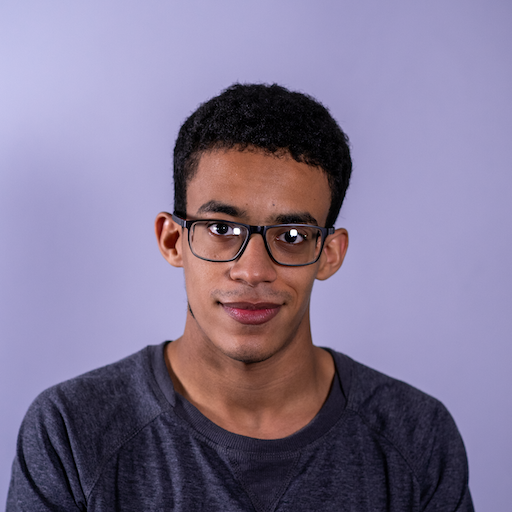
\includegraphics[]{images/Anier_Velasco.png}
%     \end{center}
% \end{figure}

%----------------------------------------------------------------------------------------
%	WORK EXPERIENCE
%----------------------------------------------------------------------------------------

\section{Work Experience}

% Each job is added with a \jobentry command. Below is an empty one to use as a template:

%\jobentry
%	{} % Duration
%	{} % FT/PT (full time or part time)
%	{} % Employer
%	{} % Job title
%	{} % Description

% All 5 parameters must be supplied but any can be empty if you don't need them

%------------------------------------------------

\jobentry
	{Current, from July 2021} % Duration
	{PT} % FT/PT (full time or part time)
	{leaguesofcode.com} % Employer
	{Backend Software Developer} % Job title
	{I'm part of the back-end team that is building an E-learning platform, with an automatic grading system for training the next generations of champions in International Programming Olympiads.
    } % Description

%------------------------------------------------

\jobentry
	{} % Duration
	{} % FT/PT (full time or part time)
	{Freelancing} % Employer
	{Tutor} % Job title
	{I teach programming, mathematics, algorithms, and competitive programming to students from High School to University.
    } % Description

%----------------------------------------------------------------------------------------
%	EDUCATION
%----------------------------------------------------------------------------------------

\section{Education} 

% Each qualification entry is added with a \qualificationentry command. Below is an empty one to use as a template:

%\qualificationentry
%	{} % Duration
%	{} % Degree
%	{} % Honors, achievements or distinctions (e.g. first class honors)
%	{} % Department
%	{} % Institution

% All 5 parameters must be supplied but any can be empty if you don't need them

%------------------------------------------------

\begin{supertabular}{r l} % Start a table with two columns, the table will ensure everything is aligned

	%------------------------------------------------
	
	\qualificationentry
		{2020 -- 2023} % Duration
		{Bachelor of Science} % Degree
		{} % Honors, achievements or distinctions (e.g. first class honors)
		{Computer Science} % Department
		{Harbour.Space University} % Institution
	
	%------------------------------------------------

\end{supertabular}

\section{Machine Learning Courses} 

% This section is laid out using a table. A \tableentry command adds lines with the following parameters:

%\tableentry{Heading}{Content}{spaceafter}
% All 3 parameters must be supplied but any can be empty if you don't need them
% A "spaceafter" value in the third parameter will add some vertical space -- tis is to be used between headings, leave it empty for no extra space

%------------------------------------------------

\begin{supertabular}{r l} % Start a table with two columns, the table will ensure everything is aligned
	
	%------------------------------------------------
	
	\tableentry{}{\href{https://harbour.space/data-science/courses/introduction-to-machine-learning-radoslav-neychev-480}{Intro to ML (link embedded in the text)}}{spaceafter}
	\tableentry{}{\href{https://harbour.space/computer-science/courses/text-mining-sergey-khoroshenkikh-487}{Text Mining (link embedded in the text)}}{}
	\tableentry{}{\href{https://harbour.space/data-science/courses/master-s-machine-learning-radoslav-neychev-623}{Master's ML (link embedded in the text)}}{}
	
	%------------------------------------------------
	
\end{supertabular}


\section{University Projects} 

% This section is laid out using a table. A \tableentry command adds lines with the following parameters:

%\tableentry{Heading}{Content}{spaceafter}
% All 3 parameters must be supplied but any can be empty if you don't need them
% A "spaceafter" value in the third parameter will add some vertical space -- this is to be used between headings, leave it empty for no extra space

%------------------------------------------------

\begin{supertabular}{r l} % Start a table with two columns, the table will ensure everything is aligned
	
	%------------------------------------------------
	
	\tableentry{Search Engine}{github.com/aniervs/search-engine}{spaceafter}
	
	\tableentry{Web Chat App}{github.com/aniervs/Modern-Web-Dev2}{}
	
	%------------------------------------------------
	
\end{supertabular}

%----------------------------------------------------------------------------------------
%	COMPUTER SKILLS
%----------------------------------------------------------------------------------------

\section{Technical Skills} 

% This section is laid out using a table. A \tableentry command adds lines with the following parameters:

%\tableentry{Heading}{Content}{spaceafter}
% All 3 parameters must be supplied but any can be empty if you don't need them
% A "spaceafter" value in the third parameter will add some vertical space -- this is to be used between headings, leave it empty for no extra space

%------------------------------------------------

\begin{supertabular}{r l} % Start a table with two columns, the table will ensure everything is aligned
	
	%------------------------------------------------
	
	\tableentry{Beginner}{\LaTeX, GraphQL}{spaceafter}
	
	%------------------------------------------------
	
	\tableentry{Intermediate}{Php, Laravel, MySQL}{}
	\tableentry{}{Python, C++, Unix}{}
	\tableentry{}{Machine Learning}{spaceafter}
	
	%------------------------------------------------
	
	\tableentry{Advanced}{Algorithms, Data Structures}{}
    \tableentry{}{Competitive programming}{spaceafter}
	
	%------------------------------------------------
	
\end{supertabular}


\medskip % Extra vertical whitespace before the next section

%----------------------------------------------------------------------------------------

\switchcolumn % Switch to the second (right) column

%----------------------------------------------------------------------------------------
%	COLORED CONTACT DETAILS BOX
%----------------------------------------------------------------------------------------

\parbox[top][0.11\textheight][c]{\linewidth}{ % Box to hold the colored box; change the fixed height as needed to match the box to the left
	\colorbox{shade}{ % Create colored box and specify background color
		\begin{supertabular}{@{\hspace{3pt}} p{0.05\linewidth} | p{0.775\linewidth}} % Start a table with two columns, the table will ensure everything is aligned
			\raisebox{-1pt}{\faHome} & Barcelona, Catalonia, Spain\\ % Address
			\raisebox{-1pt}{\faPhone} & +34 678 908 982 \\ % Phone number
			\raisebox{-1pt}{\small\faEnvelope} & \href{mailto:anier.velasco@gmail.com}{anier.velasco@gmail.com} \\ % Email address
			\raisebox{-1pt}{\faLinkedinSquare} & \href{https://www.linkedin.com/in/aniervs}{linkedin.com/in/aniervs} \\ % LinkedIn profile
			\raisebox{-1pt}{\faGithub} & \href{https://github.com/aniervs}{github.com/aniervs} \\ % Github profile
            % \raisebox{-1pt}{\textbf{CF}} & \href{https://codeforces.com/profile/aniervs}{codeforces.com/profile/aniervs} \\ % Codeforces profile
			% See fontawesome.pdf in the Fonts folder for all icons you can use
		\end{supertabular}
	}
	\vfill % Push content to the top of the box
}


%----------------------------------------------------------------------------------------
%	AWARDS
%----------------------------------------------------------------------------------------

\section{Programming Competitions}

% This section is laid out using a table. A \tableentry command adds lines with the following parameters:

%\tableentry{Heading}{Content}{spaceafter}
% All 3 parameters must be supplied but any can be empty if you don't need them
% A "spaceafter" value in the third parameter will add some vertical space -- this is to be used between headings, leave it empty for no extra space

%------------------------------------------------

\begin{supertabular}{r l} % Start a table with two columns, the table will ensure everything is aligned
	
	%------------------------------------------------
	
	\tableentry{2022}{\textbf{SWERC ICPC} (swerc.eu/2021/about/)}{}
	\tableentry{}{ICPC Foundation}{spaceafter}

	%------------------------------------------------
	
	\tableentry{2021}{\textbf{SWERC ICPC} (swerc.eu/2020/about/)}{}
	\tableentry{}{ICPC Foundation}{spaceafter}
	
	%------------------------------------------------
	
    \tableentry{2019 and 2018}{\textbf{2x Bronze Medal}}{}
	\tableentry{}{Iberoamerican Informatics Olympiad}{spaceafter}

    %------------------------------------------------

	\tableentry{2019 and 2018}{\textbf{2x Gold Medal}}{}
	\tableentry{}{Cuban Informatics Olympiad}{spaceafter}

    %------------------------------------------------

\end{supertabular}


%----------------------------------------------------------------------------------------
%	COMMUNICATION SKILLS
%----------------------------------------------------------------------------------------

\section{Communication Skills}

% This section is laid out using a table. A \tableentry command adds lines with the following parameters:

%\tableentry{Heading}{Content}{spaceafter}
% All 3 parameters must be supplied but any can be empty if you don't need them
% A "spaceafter" value in the third parameter will add some vertical space -- this is to be used between headings, leave it empty for no extra space

%------------------------------------------------

\begin{supertabular}{r l} % Start a table with two columns, the table will ensure everything is aligned
	
	%------------------------------------------------
	
	\tableentry{Languages}{English (fluent)}{}
	\tableentry{}{Spanish (native speaker)}{spaceafter}
	
	%------------------------------------------------
	
\end{supertabular}

%----------------------------------------------------------------------------------------
%	VOLUNTEERING
%----------------------------------------------------------------------------------------

\section{Volunteering}

\jobentry{}{}{}{Coach}{
	I volunteered as mentor of a group of high school students in a 1 week-long \href{https://vimeo.com/702917364}{Hackathon at St. Paul's School}, organized by Harbour.Space University,
	where the students needed to come out with a business idea and develop it further during week, and pitch it to real experts in entrepeurship on the last day.
}

\jobentry{}{}{}{Problemsetter}{	
	- Cuban Olympiad in Informatics 2022 (OCI 2022).

	- Iberoamerican Olympiad in Informatics 2020 (CIIC 2020).
}
%----------------------------------------------------------------------------------------
%	REFERENCES
%----------------------------------------------------------------------------------------

\section{References}

% \textit{References available on request} % Uncomment if you'd rather not include references and remove the section below

%------------------------------------------------

% This section is laid out using a table. A \tableentry command adds lines with the following parameters:

%\tableentry{Heading}{Content}{spaceafter}
% All 3 parameters must be supplied but any can be empty if you don't need them
% A "spaceafter" value in the third parameter will add some vertical space -- this is to be used between headings, leave it empty for no extra space

%------------------------------------------------

\begin{supertabular}{r l} % Start a table with two columns, the table will ensure everything is aligned
	
	%------------------------------------------------
	
	% \\ % Additional vertical whitespace between the references
	
	%------------------------------------------------
	
	\tableentry{}{\textbf{Konstantin Mertsalov}}{spaceafter}
	\tableentry{Position}{PhD, Director of Software Development Europe}{}
	\tableentry{Employer}{https://www.rationalenterprise.com}{spaceafter}
	\tableentry{Email}{\href{mailto:konstantin.mertsalov@harbour.space}{konstantin.mertsalov@harbour.space}}{}
	\tableentry{Telegram}{\href{https://t.me/kmertsalov}{https://t.me/kmertsalov}}{}
	
	%------------------------------------------------
	
\end{supertabular}

%----------------------------------------------------------------------------------------

\end{paracol} % End two-column mode

%----------------------------------------------------------------------------------------

\pagebreak

\end{document}
